\chapter{随机抽样}

上一章我们讨论了最简单的随机分布,均匀分布随机数的产生方法。有了这个均
匀分布随机数的基础,这一章我们将进一步讨论如何产生各种所需的随机变量和
随机过程。首先我们回顾一下概率论的一些基本定义。

\section{基础知识回顾}
我们用概率分布来描述一个随机变量服从的分布规律,具体来说,离散型随机变
量的概率分布称为

\begin{definition} {\hei 概率质量函数(Probability Mass Function, PMF)}
  若离散型随机变量$\xi$取值为$x_1, x_2, \cdots, x_n$的概率分别为$p_1,
  p_2, \cdots, p_n$, 即
  \begin{equation}
    P(\xi = x_i) = p_i, i = 1, 2, \cdots, n,
    \label{eq::dis_df}
  \end{equation}
  则其概率分布函数
  \begin{equation}
    f(x) = \left\{
    \begin{array}{ll}
      p_i, & x \in S,\\
      0, & x \in \mathbb{R}\setminus S
    \end{array}\right.
    \label{eq::dis_pmf}
  \end{equation}
  又称为概率质量函数,简称为PMF。其中$S = \{x_1, x_2, \cdots, x_n\}$称
  为样本集。显然,在离散的情形下,有
$$
\sum_{x_i \in S}p_i = \sum_{i = 1}^np_i = 1.
$$
\label{def::dis_pmf}
\end{definition}


\begin{definition} {\hei 累积分布函数(Cumulative Distribution Function, CDF)}
  称
  \begin{equation}
    F(x) = P(\xi \leq x) = \sum_{x_i \leq x}p_i, x \in \mathbb{R}
    \label{eq::dis_cdf}
  \end{equation}
  为累积分布函数,简称为CDF。
  \label{def::dis_cdf}
\end{definition}

\begin{example} {\hei 两点分布} 最简单的两点分布的PMF为
  \begin{equation}
    f(x) = \left\{\begin{array}{ll}
    0.5, &x = 0; \\
    0.5, &x = 1;\\
    0, &x \notin \{0, 1\}.
    \end{array}\right.
    \label{eq::2p_PMF}
  \end{equation}
  对应的CDF为
  \begin{equation}
    F(x) = \left\{\begin{array}{ll}
    0, & x < 0; \\
    0.5, &0 \leq x < 1; \\
    1, &x = 1.
    \end{array}\right.
    \label{eq::2p_CDF}
  \end{equation}
  \label{example::2p}
\end{example}

更常见的,离散型随机变量的特征会像下面那样表示。

\begin{example} {\hei 二项分布} 的PMF一般写做
\begin{equation}
  b(k; n, p) = \binom{n}{k}p^k(1 - p)^{n - k}, 0 < p < 1, k = 0, 1, \cdots, n.
  \label{eq::binom_PMF}
\end{equation}
\label{example::binom}
\end{example}

我们考虑$n = 10$,$p = 0.3$的特例,我们可以根据其PMF给出对应的二项分布
表\ref{table::df_bin},以及对应的图\ref{fig::DF_bin}。

\begin{table}[!ht]
  \centering
  \caption{二项分布表,$n = 10$,$p = 0.3$}
  \label{table::df_bin}
\begin{tabular}{|c|c|c|c|}
  \hline
  $k$&0&1\\
  \hline
  $P(\xi = k)$&0.028247524900000005&0.12106082100000018\\
  \hline
  $k$&2&3\\
  \hline
  $P(\xi = k)$&0.2334744405&0.26682793200000016\\
  \hline
   $k$&4&5\\
   \hline
   $P(\xi = k)$&0.20012094900000013&0.10291934520000007\\
   \hline
   $k$&6&7\\
   \hline
   $P(\xi = k)$&0.03675690899999999&0.009001692000000002\\
   \hline
   $k$&8&9\\
   \hline
   $P(\xi = k)$&0.0014467004999999982&0.00013778100000000015\\
   \hline
   $k$&10&\\
   \hline
   $P(\xi = k)$&5.904899999999995e-06& \\
   \hline
\end{tabular}
\end{table}

\begin{figure}[!ht]
\centering
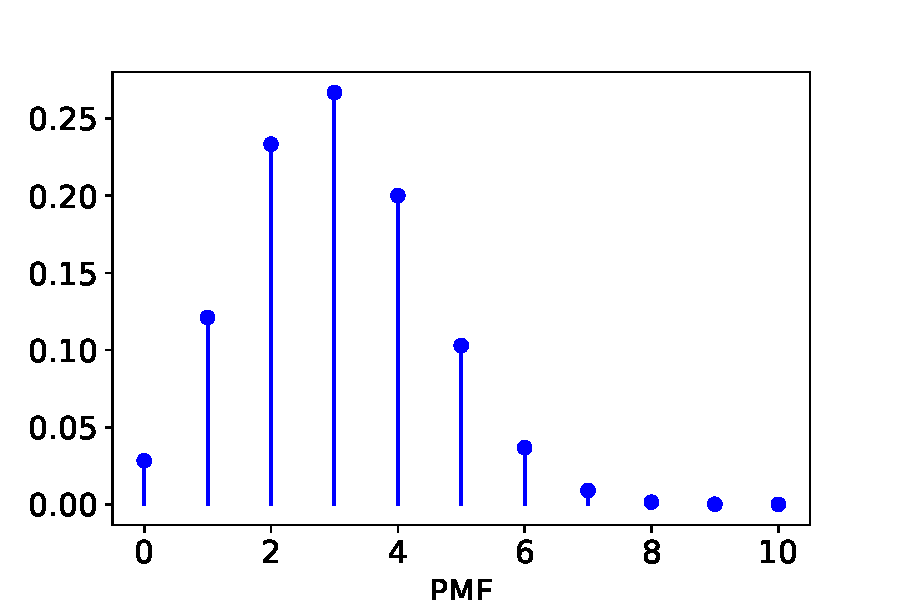
\includegraphics[width=0.45\textwidth]{images/PMF_bin.pdf}
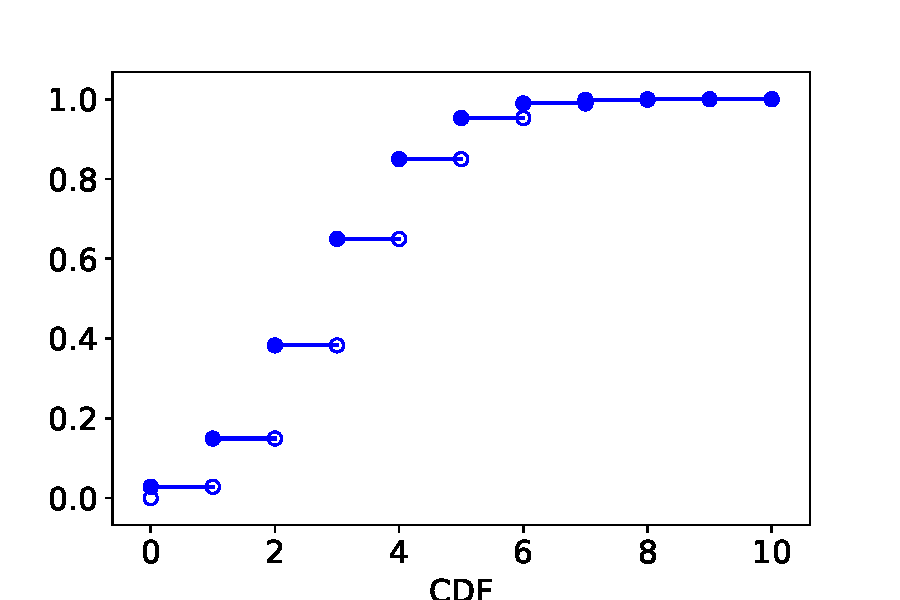
\includegraphics[width=0.45\textwidth]{images/CDF_bin.pdf}
\caption{二项分布,$n = 10$,$p = 0.3$,左:PMF,右:CDF。}
\label{fig::DF_bin}
\end{figure}

随机模拟的一个重要步骤是根据需要产生服从各种分布的样本集。之前我们已经
讨论过如何产生服从$U(0, 1)$的均匀分布的随机数,那么现在,我们就要从服
从$U(0, 1)$的均匀分布的随机序列出发,产生独立同分布的目标随机数序列。
这里两个问题的解决是各自独立的。首先随机序列的独立性完全由均匀分布的随
机序列的独立性决定,这在上一章已经讨论。我们接下去主要讨论如何确保随机
序列同分布,也即和要求的目标分布一致。这里还有一个重要问题是产生效率,
因为我们必须在计算机上算法实现。

\section{直接抽样方法}
如果随机变量的PMF是已知的,那么我们可以从均匀分布的随机数出发,直接根
据概率论定义构建抽样算法。这种方法称为直接抽样方法。即产生均匀分布的随
机序列,然后通过某种变换或抽取,使得从中变换抽取后的随机数样本集$X$服
从$F(x)$,这里$F(x)$是已知积累分布函数。也即要求$\forall \xi \sim F$,
\begin{equation}
  P(\xi \leq x) = F(x), x \in \mathbb{R}.
  \label{eq::def_cdf}
\end{equation}
这里,一方面,我们要从算法保证(证明)$X$确实服从指定分布$F(x)$;另
一方面,对于一个实际的产生的抽样结果,也要能通过指定的统计检验。

\subsection{逆变换算法}

1947年,曼哈顿计划的参与者Stanislaw Marein Ulam提出了逆变换算法,注意
到随机变量$\xi$的累积分布函数$F(x): \mathbb{R} \mapsto [0, 1]$是非降
的,故定义其逆函数为
\begin{equation}
  F^{-1}: [0, 1] \mapsto \mathbb{R}, F^{-1}(y) = \inf \{x \left| F(x)
  \geq y \right.\}
  \label{eq::inv_cdf}
\end{equation}

\begin{theorem}{}
  若随机变量$\eta$服从$[0, 1]$上的均匀分布,$F(x)$是指定分布的CDF,令
  $\xi = F^{-1}(\eta)$,则$\xi$服从$F(x)$.

  \noindent{\hei 证明:} $\forall x \in \mathbb{R}$,
  \begin{equation}
    P(\xi \leq x) = P(F^{-1}(\eta) \leq x) = P(\eta \leq F(x)) = F(x).
    \label{eq::prof_inv_cdf}
  \end{equation}
  证毕.
  \label{thm::inv_cdf}
\end{theorem}

所以我们算法的设计思路就是对一个均匀分布的随机数序列$U$,求其逆变换$X
= F^{-1}(U)$,则$X$的分布服从$F(x)$。

\subsection{列表查找法}
这种做法一般针对离散分布,特别是能给出分布表的离散分布。若离散分布的PMF表为
$$
\begin{array}{cccc}
  x_0 & x_1 & \cdots & x_n \\
  p_0 & p_1 & \cdots & p_n,
\end{array}
$$
且$x_0 < x_1 < \cdots < x_n$, 则我们不难构建CDF表
$$
\begin{array}{cccccc}
  x_0 & x_1 & \cdots & x_k & \cdots & x_n \\
  F_0 = p_0 & F_1 = p_0 +  p_1 & \cdots
  & F_k = \sum_{i = 0}^k p_i & \cdots & F_n \equiv 1.
\end{array}
$$
根据定义\ref{def::dis_pmf},$\forall x \notin \{x_0, x_1, \cdots,
x_n\}$,有$f(x) = 0$,故我们可以认为$F_{-1} = 0$。现在对$\eta \sim U(0, 1)$,
必有$0 \leq k \leq n$(为什么?), 满足
\begin{equation}
  \label{eq::def_dis_pmf}
F_{k - 1} < \eta \leq F_k,
\end{equation}
则可取$\xi = x_k$。从PMF角度,就是
\begin{equation}
  \xi = \min\left\{x_k\left|\eta \leq \sum_{i = 0}^kf(x_i)\right.\right\}, \eta \sim U(0, 1).
  \label{eq::dis_inv}
\end{equation}
在具体的抽取算法中,这一过程就是查表。对于较长的表,应该注意采用二分查
找(不知为何经典教材都是顺序遍历,大家仔细想想我有没有bug?)。具体算
法见算法\ref{alg::dis_sample_table}。

\begin{minipage}[!ht]{0.8\textwidth}
\vspace{3ex}
\refstepcounter{alg}
\label{alg::dis_sample_table}
\begin{center}
 算法 \arabic{chapter}.\arabic{alg} 离散随机分布的查表抽样
\end{center}
\small
\begin{tabular}{lll}
  \hei 输入&F&CDF\\
  &eta&$U(0,1)$分布的随机变量\\
  &start&起始抽样点\\
  &end&终止抽样点\\
  \hei 输出&&服从F分布的随机变量
\end{tabular}
\begin{lstlisting}[style = python]
def bisection_search(F, eta, start, end):
    if (eta <= F[start]):
        return start
    n = end - start
    if (n <= 0):
        sys.exit()
    k = (start + end) // 2
    if (eta > F[k]):
        if (eta <= F[k + 1]):
            return k + 1
        else:
            return bisection_search(F, eta, k + 1, end)
    else:
        return bisection_search(F, eta, start, k)
\end{lstlisting}
\end{minipage}

图\ref{fig::dis_bin_stat}给出了对$n = 10, p = 0.3$的二项分布的100万次抽样的统计检验结果。可以看到统计结果和理论PMF符合的很好。

\begin{figure}[!ht]
\centering
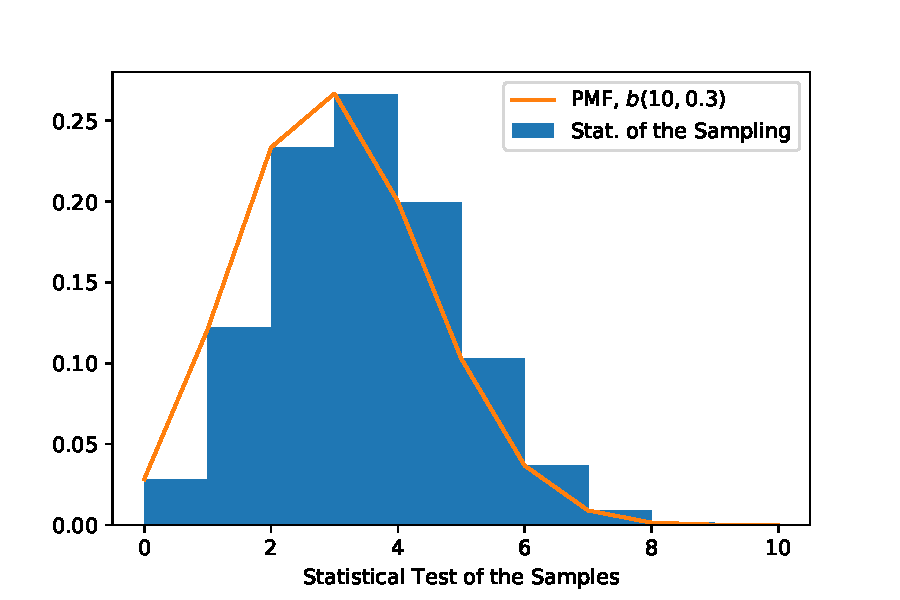
\includegraphics[width=0.7\textwidth]{images/test_bin.pdf}
\caption{对算法\ref{alg::dis_sample_table}抽样生成的$n = 10$,$p =
  0.3$二项分布的统计检验。柱状图是对100万次抽样生成样本集分布的统计,
  折线是$b(10, 0.3)$的PMF。二者吻合一致。}
\label{fig::dis_bin_stat}
\end{figure}


\subsection{连续分布的情形}
而对于连续型随机变量,可以看作是离散型随机变量的一种极限情形。此时概率
分布无法逐点定义,而是定义在样本集内的正测度集上,即考察随机变量落在一
个正测度集内的概率是多少。而从这个角度我们发现,之前在定义
\ref{def::dis_cdf}所引入的累积分布函数
$$
F(x) = P(\xi \leq x), x \in \mathbb{R}
$$
对连续型随机变量仍然适用,而在此基础上,可进一步引入直观上``概率如何
在一点上的定义''。由于一点是零测度集,所以这种定义无法脱离正测度集的概
念独立存在,而被看作``微元正测度集''的概率。

\begin{definition} {\hei 概率密度函数(Probability Density Function, PDF)}
  对连续型随机变量,$\forall x \in \mathbb{R}$, 我们仍称
  \begin{equation}
    F(x) = P(\xi \leq x), x \in \mathbb{R}
    \label{eq::df}
  \end{equation}
  为累计分布函数,若存在某个非负的可积函数$f(x)$,满足
  \begin{equation}
    F(x) = \int_{-\infty}^x f(y) dy, \forall x \in \mathbb{R},
    \label{eq::pdf}
  \end{equation}
  则称$f(x)$为对应随机分布的概率密度函数,简称为PDF。此时,
  \begin{equation}
    f(x) = F'(x).
    \label{eq::pdf2cdf}
  \end{equation}
  \label{def::pdf}
\end{definition}
注意到我们之前定义的针对离散型随机变量的PMF,事实上和这里定义的PDF
并无冲突,甚至可以看作是PDF的一个特例(这里要看你如何定义积分了)。关
于逆变换的定义也可以完全沿用。

\renewcommand\arraystretch{1.5}
\begin{table}[!ht]
  \centering
  \caption{常用连续概率分布的PDF和逆变换}
  \label{table::pdf_inv}
\begin{tabular}{|l|l|l|}
  \hline
  概率分布&PDF&逆变换\\
  \hline
  \small 均匀分布&$\frac{1}{b - a}, x \in [a, b]$&$a + (b - a)y$\\
  \hline
  \small Rayleigh分布&$\frac{x}{\sigma^2}e^{-\frac{x^2}{2\sigma^2}}, x > 0$
  &$\sqrt{-2\sigma^2\ln y}$\\
  \hline
  \small 指数分布&$\frac{1}{\lambda} e^{-\frac{x}{\lambda}}, \lambda > 0, x \geq 0$
  &$-\lambda\ln y$\\
  \hline
  \small Weibull分布&$\frac{a}{b^a}x^{a - 1} e^{-\left(\frac{x}{b}\right)^a},
  a, b > 0, x \geq 0$
  &$b\left(-\ln y\right)^{\frac{1}{a}}$\\
  \hline
  \small Beta分布&$ax^{a - 1}, a > 0, x \in [0, 1]$&$y^{\frac{1}{a}}$\\
  \hline
  \small Beta分布&$b(1 - x)^{b - 1}, b > 0, x \in [0, 1]$&$1 - y^{\frac{1}{b}}$\\
  \hline
  \small 逻辑分布&$\frac{e^{-\frac{x - a}{b}}}{b\left[1 + e^{-\frac{x - a}{b}}\right]^2}, b > 0$&$a + b \ln\left[\frac{y}{1 - y}\right]$\\
  \hline
  \small Cauchy分布&$\frac{b}{\pi\left[b^2 + (x - a)^2\right]}$
  &$a + \frac{b}{\tan(\pi y)}$\\
  \hline
  \small 正态分布&$\frac{1}{\sqrt{2\pi\sigma^2}}e^{-\frac{(x - \mu)^2}{2\sigma^2}}$&*\\
  \hline
  \small Pareto分布&$\frac{ab^a}{x^{a + 1}}, x \geq b > 0, a > 0$&$\frac{b}{(1 - y)^{\frac{1}{a}}}$\\
  \hline
\end{tabular}
\end{table}
\renewcommand\arraystretch{1}

对于连续分布的采样抽取,如果存在容易计算的逆变换解析表达式$F^{-1}(y)$,
那么对于$U(0, 1)$的均匀分布的随机变量$\eta$,直接计算$F^{-1}(\eta)$即
可。也就是说,
\begin{equation}
  \xi = \min\left\{x \left|\eta \leq \int_{-\infty}^x f(t)
  dt\right.\right\} = F^{-1}(\eta), \eta \sim U(0, 1),
  \label{eq::inv}
\end{equation}
则$\xi \sim f(x)$。算法\ref{alg::sample_inv_method}给出了Rayleigh分布
逆变换抽样的实现。

\begin{minipage}[!ht]{0.8\textwidth}
\vspace{3ex}
\refstepcounter{alg}
\label{alg::sample_inv_method}
\begin{center}
 算法 \arabic{chapter}.\arabic{alg} Rayleigh分布的逆变换抽样
\end{center}
\small
\begin{tabular}{lll}
  \hei 输入&U&$U(0, 1)$分布的随机序列\\
  &sigma&Rayleigh分布参数\\
  \hei 输出&&服从Rayleigh分布的浮点随机数组
\end{tabular}
\begin{lstlisting}[style = python]
def sample_Rayleigh(U, sigma):
    return [np.sqrt(-2 * sigma**2 * np.log(u)) for u in U]
\end{lstlisting}
\end{minipage}

\begin{figure}[!ht]
\centering
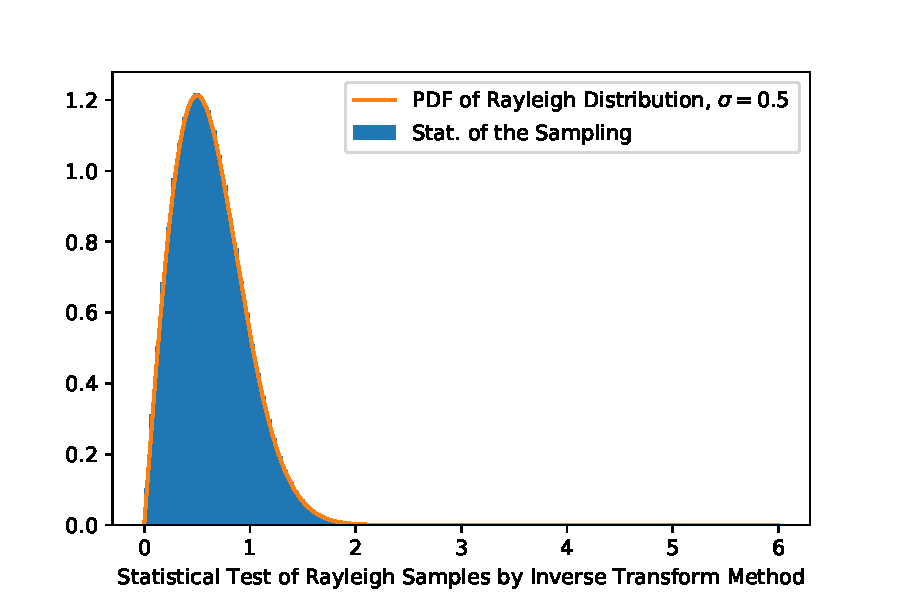
\includegraphics[width=0.7\textwidth]{images/Ray_inv.pdf}
\caption{对算法\ref{alg::sample_inv_method}抽样生成的Rayleigh分布
  ($\sigma = 0.5$)的统计检验。柱状图是对100万次抽样生成样本集分布的
  统计,折线是Rayleigh的PDF。二者吻合一致。}
\label{fig::Ray_stat}
\end{figure}

图\ref{fig::Ray_stat}给出了Rayleigh分布($\sigma = 0.5$)的采样结果和
PDF的对比。可以看到对于能快速计算逆变换的分布,这种方法是最直接的采样
手段。表\ref{table::pdf_inv}给出了一些常见分布的PDF以及相应的逆变换表
达式。从表上我们就发现并不是每一个能写出表达式的逆变换在计算上都是高效
率的,而有的甚至根本没有解析形式。比如最重要的正态分布我们就没有解析的
逆变换形式。不过Hastings 1955\cite{Hastings1955Approximations}(这是一
  本神奇的书,给出了各种难以计算公式的有理逼近估计)给出了一个有理逼近
形式:
\begin{equation}
  F^{-1}(y) = \mu
  + \mathrm{sign}(y - \frac{1}{2})\sigma\left(t
  - \frac{c_0 + c_1 t + c_2 t^2}{1 + d_1 t + d_2 t^2 + d_3 t^3}\right),
  \label{eq::approx_normal}
\end{equation}
其中
$$
t = \sqrt{-\ln\left[\min(y, 1 - y)\right]^2},
$$
各参数值为
$$
\begin{array}{c}
  c_0 = 2.515517, c_1 = 0.802853, c_2 = 0.010328,\\
  d_1 = 1.432788, d_2 = 0.189269, d_3 = 0.001308.
\end{array}
$$
此公式绝对误差小于$0.45 \times 10^-3$。

如果逆变换本身没有解析形式或者难以计算,那么另一个方法是直接从CDF入手
计算(注意不是PDF),当然前提是PDF和CDF可以快速计算。这本质上就是之前
离散的情况的查表的极限沿拓,到了连续情形就变成对一个$\forall y \in [0,
1]$,寻找$x \in \mathbb{R}$,满足
\begin{equation}
  F(x) = y \Rightarrow F(x) - y = 0.
  \label{eq::inv_equation}
\end{equation}
而上述方程,我们可以用数值方法,比如二分法,或Newton法求解。

\section{取舍算法}

总是有一些分布,或者写不出反函数的解析表达,或者该解析表达难以计算(或
  计算量很大)。比如最重要的正态分布就没有显式的积累分布函数的解析表达。
而一些初等函数,如指数,对数的计算,事实上计算量是极大的。1947年,冯·
诺伊曼\cite{von195113}从条件概率入手,提出了取舍算法(Accept-Rejection
Method,简称AR法)。

\begin{theorem} (von Neumann 1951)
令$f(z)$,$a \leq z \leq b$是某分布的概率密度函数且具有分解形式
  \begin{equation}
    f(z) = c g(z) h(z),
    \label{eq::AR_frac_pdf}
  \end{equation}
  其中
  \begin{equation}
    h(z) \geq 0, \int_a^b h(z) dz = 1, c = \sup_{z}\left[\frac{f(z)}{h(z)}\right],
    \label{eq::AR_pfd_hc}
  \end{equation}
  并且
  \begin{equation}
    0 \leq g(z) \leq 1.
    \label{eq::AR_pdf_g}
  \end{equation}
  令$Z$是PDF为$h(z)$的随机变量,$U$为服从$U(0, 1)$的随机变量。
  则满足$U \leq g(Z)$的随机变量$Z$服从PDF为$f(z)$的概率分布。
  \label{thm::AR}
\end{theorem}

\begin{proof}
随机变量$U$的PDF为$1$,$u \in [0, 1]$;而$Z$的PDF为$h(z)$,$z \in [a, b]$,
  故二者联合分布,即随机向量$(U, Z)$的PDF为
  \begin{equation}
    f_{U, Z}(u, z) = h(z).
  \end{equation}
  (不严格地,可看作任取$[0, 1] \times [a, b]$中的一点,事件恰好落在这
    一点的概率。把点想像成一个点微元。)
现在考虑$Z$的条件概率分布
  \begin{equation}
    h_Z(z\left|U \leq g(Z)\right.) =
    \frac{\int_0^{g(z)}f_{U, Z}(u, z)du}{P(U \leq g(Z))}.
    \label{eq::AR_cond_h}
  \end{equation}
(这个事件说的是,首先$Z$是一个随机变量,它按$h(Z)$的概率分布发生。然
  后$U$是一个$U(0, 1)$分布的随机变量。两件事情同时发生的概率,可以认为
  是先有$h(Z)$的概率$Z$落在了$z$点,我们还是把它想像成一个微元事件,同
  时$U$落在$[0, g(z)]$区间上,可以是其中任何一点,所以要积分。这两件事
  情的全概率是上式的分子。现在我们求的条件概率是,如果$U$和$Z$各自都是
  独立的,$U$在投点的时候并不知道$Z$在哪里,以及$g(Z)$是多少,但我们还
  是想问这种情况下,$U \leq g(Z)$的这个事件,关于$Z$的概率密度分布是多
  少?那么这个就是条件概率分布,它要除以$U \leq g(Z)$的概率。)
  
  再由(因为$f(z)$是PDF)
  \begin{equation}
    c = \frac{1}{\int_{a}^b g(z) h(z)dz},
    \label{eq::AR_dri_c}
  \end{equation}
  以及
  \begin{equation}
    \int_0^{g(z)}f_{U, Z}(u, z)dx = \int_0^{g(z)} h(z) du = g(z) h(z),
    \label{eq::AR_cond_f}
  \end{equation}
  和
  \begin{equation}
    P(U \leq g(Z)) = \int_{a}^b h (z) g(z) dz = \frac{1}{c},
    \label{eq::AR_conf_f_bottom}
  \end{equation}
($Z$落在$z \in [a, b]$点的概率是$h(z)$,然后此时$U < g(Z)$的概率就是
  $g(z)$,故$Z$落在$z$点,同时$U < g(Z)$的单点微元概率是$h(z)g(z)$,对
  $Z$取遍全部可能性积分,就得到全部可能的概率。注意和上面分子的不同。
  分子求的是一个边际分布,是一个关于$Z$的概率密度分布,而分母是一个概
  率,是一个数。在条件概率公式下,构成了所求的条件概率密度分布函数。)
  最终有
  \begin{equation}
    h_Z(z\left|U \leq g(Z)\right.) = c g(z) h(z) = f(z).
    \label{eq::dri_f}
  \end{equation}
\end{proof}

%% \begin{theorem} (von Neumann 1951) 令$f(x), x \in \mathbb{R}$
%%   是某分布的概率密度函数且具有分解形式
%%   \begin{equation}
%%     f(x) = c g(x) h(x),
%%     \label{eq::AR_frac_pdf}
%%   \end{equation}
%%   其中
%%   \begin{equation}
%%     h(x) \geq 0, \int_{-\infty}^\infty h(x) dx = 1, c = \sup_{x}\left[\frac{f(x)}{h(x)}\right],
%%     \label{eq::AR_pfd_hc}
%%   \end{equation}
%%   并且
%%   \begin{equation}
%%     0 \leq g(x) \leq 1.
%%     \label{eq::AR_pdf_g}
%%   \end{equation}
%%   令$\xi$是PDF为$h(x)$的随机变量,$\eta$为服从$U(0, 1)$的随机变量。
%%   则满足$g(\xi) \geq \eta$的$\xi$服从概率密度分布$f(x)$。

%%   {\hei 证明} 注意到随机向量$(\eta, \xi)$的联合分布为:
%%   \begin{equation}
%%     f_{\eta, \xi}(x, y) = h(y), 0 \leq x \leq 1, y \in \mathbb{R}.
%%     \label{eq::AR_uni_f}
%%   \end{equation}
%%   于是条件分布:
%%   \begin{equation}
%%     h_\xi(y\left|\eta \leq g(\xi)\right.) =
%%     \frac{\int_0^{g(y)}f_{\eta, \xi}(x, y)dx}{P(\eta \leq g(\xi))}.
%%     \label{eq::AR_cond_h}
%%   \end{equation}
%%   再由(因为$f(x)$是PDF)
%%   \begin{equation}
%%     c = \frac{1}{\int_{-\infty}^\infty g(x) h(x)dx},
%%     \label{eq::AR_dri_c}
%%   \end{equation}
%%   以及
%%   \begin{equation}
%%     \int_0^{g(y)}f_{\eta, \xi}(x, y)dx = \int_0^{g(y)} h(y) dx = g(y) h(y),
%%     \label{eq::AR_cond_f}
%%   \end{equation}
%%   和
%%   \begin{equation}
%%     P(\eta \leq g(\xi)) = \int_{-\infty}^\infty h (y) g(y) dy = \frac{1}{c},
%%     \label{eq::AR_conf_f_bottom}
%%   \end{equation}
%%   最终有
%%   \begin{equation}
%%     h_\xi(y\left|\eta \leq g(\xi)\right.) = c g(y) h(y) = f(y).
%%     \label{eq::dri_f}
%%   \end{equation}
%%   证毕.
%%   \label{thm::AR}
%% \end{theorem}

根据定理结果,如果我们已知$g(z)$和$h(z)$,则可以构建算法产生服从分布
$f(z)$的随机变量。基本步骤为:
\begin{enumerate}
\item 产生服从分布$h(z)$的随机变量$Z$;
\item 产生服从$U(0, 1)$的随机变量$U$;
\item 计算$g(Z)$;
\item 若$U \leq g(Z)$,返回$Z$,否则放弃,返回第1步.
\end{enumerate}

\begin{example} 标准半正态分布(half-normal distribution)的PDF为:
  \begin{equation}
    f(z) = \sqrt{\frac{2}{\pi}} e^{\frac{-z^2}{2}}, 0 \leq z < \infty.
    \label{eq::def_half_normal}
  \end{equation}
  我们可以将其写作
  \begin{equation}
    f(z) = \sqrt{\frac{2e}{\pi}} e^{-\frac{-(z - 1)^2}{2}}e^{-z},
    \label{eq::frac_half_normal}
  \end{equation}
  并令
  \begin{eqnarray}
    h(z) &=& e^{-z}, \\
    \label{eq::half_normal_h}
    g(x) &=& e^{\frac{-(z - 1)^2}{2}},
    \label{eq::half_normal_g}
  \end{eqnarray}
  以及
  \begin{equation}
    c = \sqrt{\frac{2e}{\pi}} \approx 1.3155.
    \label{eq::half_normal_c}
  \end{equation}
  \label{example::half_normal}
\end{example}

相应的,我们可以构建算法\ref{alg::sample_harl_normal}, 产生标准半正态分布。

\begin{minipage}[!ht]{0.8\textwidth}
\vspace{3ex}
\refstepcounter{alg}
\label{alg::sample_harl_normal}
\begin{center}
 算法 \arabic{chapter}.\arabic{alg} AR法抽取标准半正态分布
\end{center}
\small
\begin{tabular}{lll}
  \hei 输入&N&实际抽样总数\\
  \hei 输出&k&实际接受样本总数\\
  &X&输出服从标准半正态分布的样本(前k个有效)
\end{tabular}
\begin{lstlisting}[style = python]
def sample_half_normal(N):
    k = 0  # 实际接受总数
    U = np.random.rand(N)  # 产生均匀分布
    X = [-np.log(u) for u in U]  # 产生服从h的随机变量X
    G = [np.exp(-(x-1)**2/2) for x in X]   # 计算g(X)
    U = np.random.rand(N)  # 再次产生均匀分布
    for i in range(N):
        if U[i] <= G[i]:  # 在g发生的条件下接受
            X[k] = X[i]
            k = k + 1
    return k, X  
\end{lstlisting}
\end{minipage}

有了标准半正态分布样本集$X$,不难通过多一层均匀分布随机抽取将其变换为
标准正态分布。也即如果随机变量$\omega \sim U(0, 1)$, 遍历$x \in X$,
若$\omega \leq 0.5$,则$x = -x$,否则$x = x$. 则改造后的$X$服从标准正
态分布。这一过程应该结合在AR过程之中,完整的标准正态分布算法见算法
\ref{alg::sample_normal}。

\begin{minipage}[!ht]{0.8\textwidth}
\vspace{3ex}
\refstepcounter{alg}
\label{alg::sample_normal}
\begin{center}
 算法 \arabic{chapter}.\arabic{alg} AR法抽取标准正态分布
\end{center}
\small
\begin{tabular}{lll}
  \hei 输入&N&实际抽样总数\\
  \hei 输出&k&实际接受样本总数\\
  &X&输出服从标准正态分布的样本(前k个有效)
\end{tabular}
\begin{lstlisting}[style = python]
def sample_normal(N):
    k = 0  # 实际接受总数
    U = np.random.rand(N)  # 产生均匀分布
    X = [-np.log(u) for u in U]  # 产生服从h的随机变量X
    G = [np.exp(-(x-1)**2/2) for x in X]   # 计算g(X)
    U = np.random.rand(N)  # 再次产生均匀分布
    for i in range(N):
        if U[i] <= G[i]:  # 在g发生的条件下接受
            w = np.random.rand()
            if w <= 0.5:
                X[k] = X[i]
            else:
                X[k] = -X[i]
            k = k + 1
    return k, X
\end{lstlisting}
\end{minipage}

图\ref{fig::AR_half_and_normal}给出了标准半正态分布和正态分布的抽
样统计结果和对应的概率密度函数对比的结果,可见效果不错。

\begin{figure}[!ht]
\centering
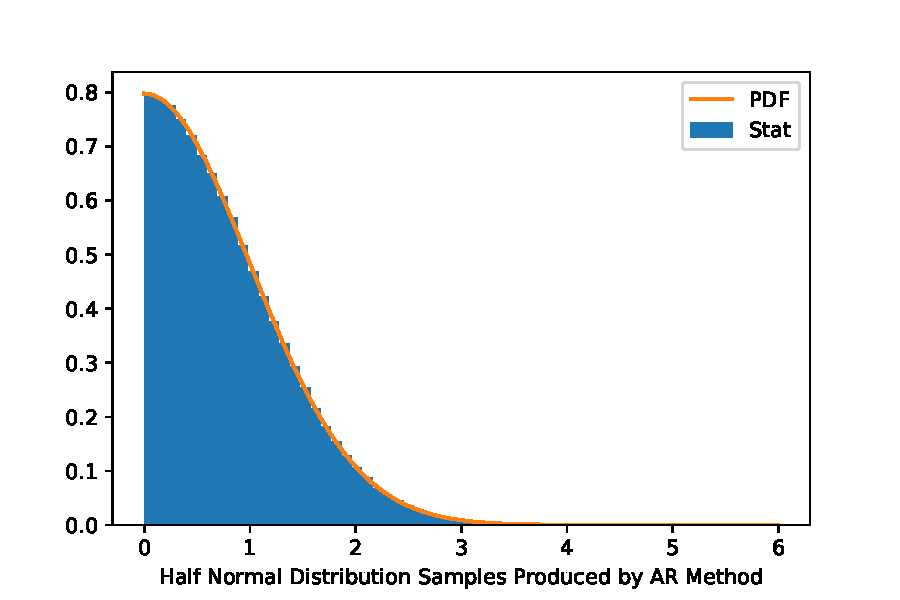
\includegraphics[width=0.45\textwidth]{images/half_normal.pdf}
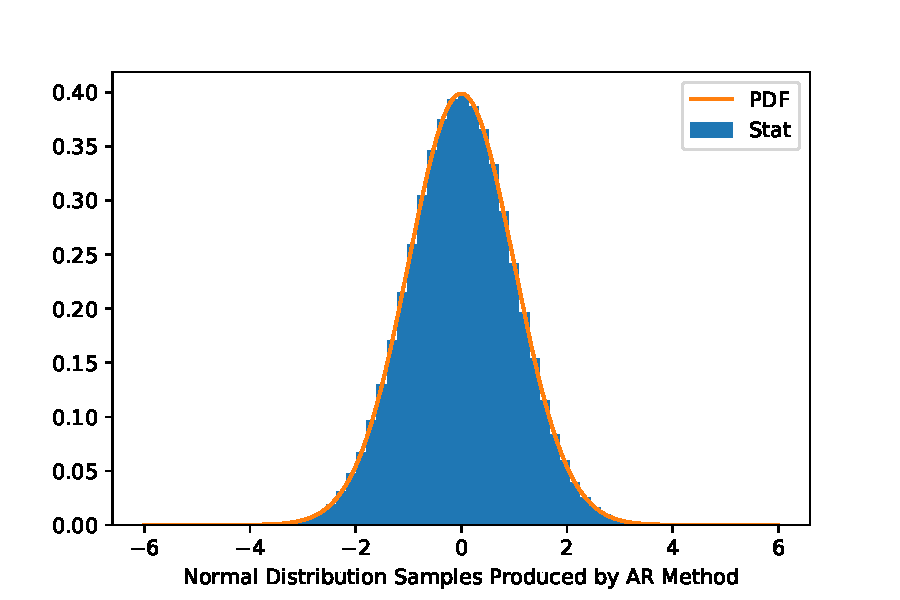
\includegraphics[width=0.45\textwidth]{images/normal.pdf}
\caption{AR法抽样生成的标准半正态分布(左,算法
    \ref{alg::sample_harl_normal})和标准正态分布(右,算法
    \ref{alg::sample_normal})的抽样统计结果和各自的PDF对比。可见抽样
  质量不错。}
\label{fig::AR_half_and_normal}
\end{figure}

我们可以如图\ref{fig::AR_region}那样绘制出用AR法抽取半正态分布的接受和
拒绝区域,它们分别是$u \leq g(-\ln x)$和$u > g(-\ln x)$,也即曲线$g(-\ln
x)$的上下部分。而常数$c$就是接受区域的面积。

注意产生目标抽样的办法肯定不止一个。我们上面严格按照AR的算法流程,先用
逆变换产生了$h$的指数分布,然后再计算$g$并通过独立的均匀分布来判定接受
或拒绝。这里产生$h$的时候用了一个log运算,产生$g$的时候做了一次指数运
算。这两个运算都是代价较高的。特别是log运算。注意到$g$本质上也是一个变
换后的指数分布,所以如果我们有一个很好的指数分布生成程序,那么可以将具
体的算法调整为各自独立地产生两个指数分布,然后对$g$产生的分布做一个变
换,再执行接受拒绝判断。具体算法见\ref{alg::sample_harl_normal_v2}。
\begin{figure}[!ht]
\centering
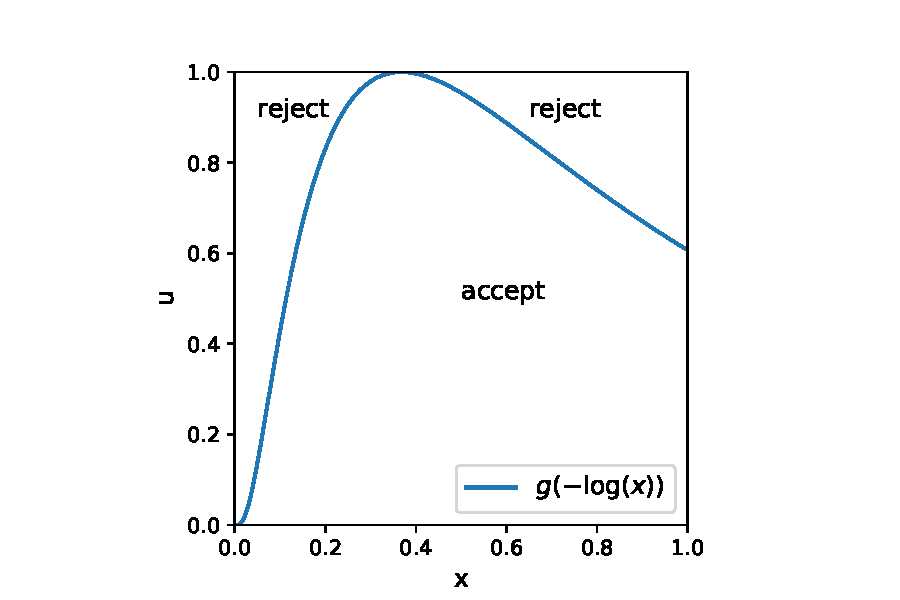
\includegraphics[width=0.7\textwidth]{images/AR_region.pdf}
\caption{AR法抽样生成的标准半正态分布的接受(accept)和拒绝(reject)区域}
\label{fig::AR_region}
\end{figure}

\begin{minipage}[!ht]{0.8\textwidth}
\vspace{3ex}
\refstepcounter{alg}
\label{alg::sample_harl_normal_v2}
\begin{center}
 算法 \arabic{chapter}.\arabic{alg} AR法抽取标准半正态分布(基于快速指
   数分布生成器)
\end{center}
\small
\begin{tabular}{lll}
  \hei 输入&N&实际抽样总数\\
  \hei 输出&k&实际接受样本总数\\
  &X&输出服从标准半正态分布的样本(前k个有效)
\end{tabular}
\begin{lstlisting}[style = python]
def sample_half_normal_v2(N):
# N, 实际采样数
    k = 0  # 实际接受总数
    X = stats.expon.rvs(size=N)  
    G = stats.expon.rvs(size=N)  # 产生两个独立的beta(1)
    for i in range(N):
        if (X[i] - 1)**2/2 <= G[i]:  # 等价于在g的条件下接受
            X[k] = X[i]   # 将采样记下来
            k = k + 1
    return k, X
\end{lstlisting}
\end{minipage}

\section{挤压算法}

我们已经注意到在抽取半正态分布时,每个样本平均需要执行
$2\sqrt{\frac{2e}{\pi}} \approx 2.631$次函数求值,一次指数运算和一次对
数运算,还得丢弃一部分。如果我们能稍微减少一些这些基本函数运算,也可以
显著降低计算代价。Marsaglia于1977年\cite{Marsaglia1977The}提出一个非常
简单但却是有效的思想,挤压算法(squeeze)。在AR法中,我们主要的计算量
来自要和$g(z)$比大小,但$g(z)$本身的计算是高代价的。如果我们能够构建关
系
\begin{equation}
  g_L(z) \leq g(z) \leq g_U(z), z \in [a, b],
\label{eq::squeeze}
\end{equation}
这里区间$[a, b]$是我们的抽样范围。而且$g_L(z)$和$g_U(z)$都是便于计算的
函数,那么对是否小于$g(z)$的判定就可以先用这两个界函数过滤一下。如果这
两个界充分接近$g(z)$,那么有很大机率,我们根本不需要再计算$g(z)$了。也
即可以将AR法的基本步骤改为:
\begin{enumerate}
\item 产生服从分布$h(z)$的随机变量$Z$;
\item 产生服从$U(0, 1)$的随机变量$U$;
\item 若$U \leq g_L(Z)$,返回$Z$;
\item 否则,若$U \leq g_U(Z)$并且$U \leq g(Z)$,返回
  $Z$,否则放弃,返回第1步。
\end{enumerate}

事实上,
\begin{equation}
  P(\mbox{计算}g(Z)) = P(g_L(Z) < U < g_U(Z)).
  \label{eq::squeeze_pg}
\end{equation}
我们用$S$表示$U \leq g(Z)$的事件,分别用$S_L$和$S_U$表示$U \leq
g_L(Z)$和$U \leq g_U(Z)$的事件,则
\begin{eqnarray}
  P(S_L) &=& \int_a^b \max\{0, g_L(z)\}h(z)dz,\\
  \label{eq::squeeze_psl}
  P(S_U) &=& \int_a^b \min\{1, g_U(z)\}h(z)dz,
  \label{eq::squeeze_psu}
\end{eqnarray}
再由\ref{eq::squeeze_pg}, 有
\begin{equation}
  P(\mbox{计算}g(Z)) = P(S_U) - P(S_L).
  \label{eq::squeeze_pg2}
\end{equation}
即在一次抽样中,要计算$g$的概率就是这么多。我们还可以令$N$为重复一次成功抽取中计算
$g(Z)$的次数,则
\begin{equation}
  E[N] = P(\bar{S}_LS_U | \bar{S})\left(\frac{1}{P(S)} - 1\right)
  + P(\bar{S}_LS_U | S).
  \label{eq::squeeze_en}
\end{equation}
这里$\bar{S}_L$和$\bar{S}$表示$U > g_L(Z)$和$U > g(Z)$,即补
事件。由条件概率公式,
\begin{equation}
  P(\bar{S}_LS_U | \bar{S}) = \frac{P(S_U) - P(S)}{1 - P(S)},
  \label{eq::squeeze_r:}
\end{equation}
和
\begin{equation}
  P(\bar{S}_LS_U | S) = \frac{P(S) - P(S_L)}{P(S)},
  \label{eq::squeeze_a}
\end{equation}
有
\begin{equation}
  E[N] = \frac{P(S_U) - P(S_L)}{P(S)}.
  \label{eq::squeeze_en_result}
\end{equation}
其中,由定义,
\begin{equation}
  P(S) = \int_a^b g(z)h(z)dz = \frac{1}{c}.
  \label{eq::squeeze_ps}
\end{equation}
用这个公式可以估计一下大概要实际抽样多少次。

经常遇到的指数和对数函数估计式如下,对指数函数,
\begin{equation}
  1 - z \leq e^{-z} \leq 1 - z + \frac{z^2}{2}, z \geq 0;
  \label{eq::squeeze_exp}
\end{equation}
对数函数
\begin{equation}
  \frac{z - 1}{z} \leq \ln z \leq -1 + z, z \geq 0.
\end{equation}

\begin{example} {\hei 对半正态抽样采用挤压法} 在算法\ref{alg::sample_harl_normal}中,我们需要计算
  $$
  g(z) = e^{-\frac{(z - 1)^2}{2}},
  $$
  现令
  \begin{equation}
    g_L(z) = 1 - \frac{(z - 1)^2}{2},
    \label{eq::squeeze_ex_gl}
  \end{equation}
  以及
  \begin{equation}
    g_U(z) = 1 - \frac{(z - 1)^2}{2} + \frac{(z - 1)^4}{8}
    = g_L(z) + \frac{(z - 1)^4}{8}.
    \label{eq::squeeze_ex_gu}
  \end{equation}
  则
  \begin{eqnarray}
    P(S_L) &=& \frac{1}{2} + (1 + \sqrt{2})e^{-(1 + \sqrt{2})} \approx 0.7159,\\
    P(S_U) &=& \frac{13}{8} - 16e^{-3} \approx 0.8284,
  \end{eqnarray}
  以及
  \begin{equation}
    P(\mbox{计算}g(Z) = P(S_U) - P(S_L) \approx 0.1125,
  \end{equation}
  同时平均每生成一个成功采样需要计算$g(z)$的次数为
  \begin{equation}
    E[N] = \frac{P(S_U) - P(S_L)}{P(S)}
    = (P(S_U) - P(S_L)) \times c \approx 0.1480.
  \end{equation}
  于是每成功生成一个采样需要计算$g(Z)$的次数从$c \approx 1.3155$下降到
  了$0.1480$,效果还是很显著的。从图\ref{fig::squeeze_half_normal}也可
  以看到需要计算$g(Z)$的范围大大减少。
  \label{example::squeeze_half_normal}
\end{example}

\begin{figure}[!ht]
\centering
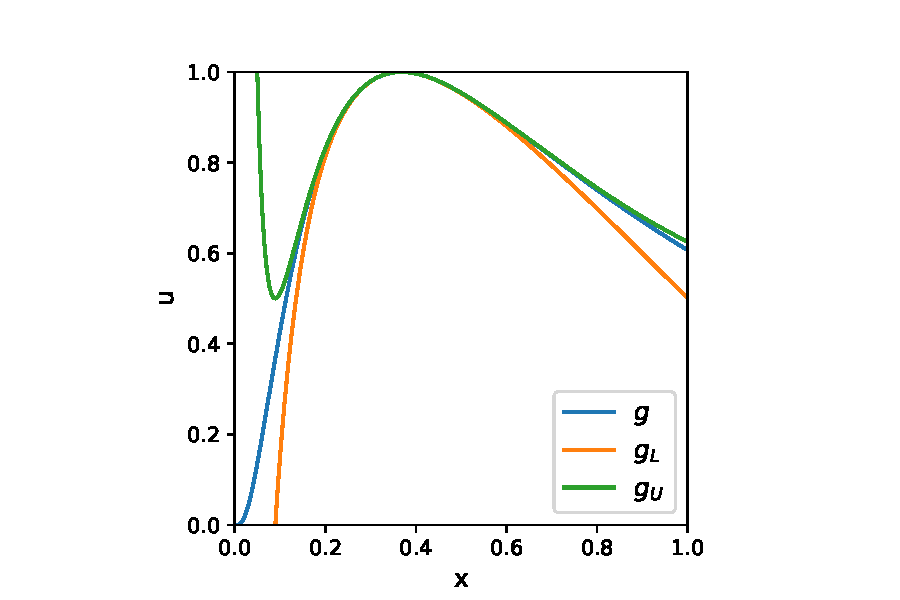
\includegraphics[width=0.7\textwidth]{images/squeeze.pdf}
\caption{用AR法抽取半正态分布,挤压后在$g_L$和$g_U$之间的区域才实际需要计算$g(Z)$。}
\label{fig::squeeze_half_normal}
\end{figure}

可以想象,高效率随机抽样这个问题既是计算机模拟的核心底层操作,又是一个
没有止境的操作。同时,和随机数生成一样,它还涉及到很多具体的理论和技术
细节。可以预见,随着计算机模拟的重要性不断提升,这些基础核心问题也会日
益受到重视。我们到这里只介绍了最基本的算法思想,更多的内容,请参阅
\cite{Fishman1995Monte}的第2 \~ 4章。同时要注意这方面不断有新文献产生。

\section{正态分布抽取}
在本章最后,我们单独介绍一个特别重要的分布的抽样方法——正态分布。服从
$N(\mu, \sigma^2)$的正态分布相应的PDF为
\begin{equation}
  f(z) = \frac{1}{\sqrt{2\pi \sigma^2}} e^{\frac{-(z -
      \mu)^2}{2\sigma^2}}, \sigma^2 > 0, z \in \mathbb{R}.
\end{equation}
关于正态分布的一些性质,大家应该是熟知的:
\begin{enumerate}
\item 若$U$服从正态分布$N(0, 1)$,
  则$Z = \mu + \sigma U$服从$N(\mu, \sigma^2)$分布;
\item 若$Z_1, Z_2, \cdots, Z_n$是分别服从$N(\mu_1, \sigma_1^2),
  N(\mu_2, \sigma_2^2), \cdots, N(\mu_n, \sigma_n^2)$的独立随机变量,
  则$Z = Z_1 + Z_2 + \cdots + Z_n$服从分布$N(\mu_1 + \mu_2 +
  \cdots + \mu_n, \sigma_1^2 + \sigma_2^2 + \cdots + \sigma_n^2)$.
\end{enumerate}
根据以上的性质,我们知道我们只需要抽样生成$N(0, 1)$就足够了。我们之前
已经介绍了如何由AR法产生半正态分布,进而抽样改造成标准正态分布。下面我
们再介绍两种简单的抽取方法。假设
\begin{equation}
  Z_n = \sqrt{12/n}(X_1 + X_2 + \cdots + X_n),
  \label{eq::normal_naive}
\end{equation}
其中$X_i$是独立的服从$U(-\frac{1}{2}, \frac{1}{2})$的随机变量,那么显然有
对$i = 1, 2, \cdots, n$, $E[X_i] = 0$, 且
$$
D[X_i] = \int_{-\frac{1}{2}}^{\frac{1}{2}}x^2 dx = \frac{1}{12}.
$$
也即$Z_n$的头两阶矩和$N(0, 1)$一致。当$n \to \infty$时,$Z_n \sim N(0,
1)$. 如果我们取$n = 12$,那么甚至连根号都不用计算了,但是这时我们发现
$Z_{12}$实际上分布在$(-6, 6)$区间而不是$\mathbb{R}$. 这个方法只有在
条件简陋的情况下可以用一下。

第二个方法可以总结成一个定理,由Box and Muller在1958年\cite{Box1958A}提出:
\begin{theorem}{}
  令随机变量$U$和$V$分别服从$U(0, 1)$和$E(1)$(表示参数为1的指数分布),那么
  \begin{equation}
    X = \sqrt{2 V}\cos 2\pi U
    \label{eq::normal_box_muller_xi}
  \end{equation}
  和
  \begin{equation}
    Y = \sqrt{2 V}\sin 2\pi U
    \label{eq::normal_box_muller_eta}
  \end{equation}
  是服从$N(0, 1)$的独立随机变量。

  \noindent{\hei 证明:} 注意到
  $$
  f_U = 1, f_V = e^{-v}.
  $$
  再令
  $$
  x = \sqrt{2v}\cos 2\pi u, y = \sqrt{2v}\sin 2\pi u,
  $$
  则有  
  $$
  2 v = x^2 + y^2
  $$
  和
  $$
  \tan 2 \pi u =\frac{y}{x}.
  $$
  因此$X$和$Y$的联合分布函数为
  \begin{equation}
    f_{X, Y}(x, y) = f_{U, V}(u(x, y), v(x,
    y))\left|\frac{\partial u}{\partial x}\frac{\partial v}{\partial
      y} - \frac{\partial u}{\partial y}\frac{\partial v}{\partial
      x}\right| = \frac{1}{2 \pi}e^{-\frac{x^2 + y^2}{2}}.
  \end{equation}
  则$f_X$和$f_Y$各自的边界分为标准正态分布。证毕。
  \label{thm::normal_box_muller}
\end{theorem}

而当前已知生成正态分布最快的方法是由Marsaglia在1964年
\cite{Marsaglia1964A}提出的rectangle-wedge-tail方法,并在1972年由
Ahrens和Dieter修改成RT算法\cite{Dieter1973A}。但是他们的方法都需要准备
大量的预制表格,这一系方法实现比较繁琐。在不用查表的情况下,生成正态分
布最快的方法,它是由Ahrens和Dieter在1988年提出的NA算法
\cite{Ahrens1988Efficient}。有兴趣的同学可自行参阅相应文献。
